\graphicspath{{./chapters/01/assets/}}
\chapter{Contesto Aziendale}
\label{cha:intro}

Reply è una società specializzata in consulenze, \textit{system integration} e servizi digitali con un focus sulla concezione, design e implementazione di soluzioni basate sulle nuove tecnologie e i nuovi canali di comunicazione. Operativa dal 1996, collabora con importanti realtà aziendali di diversi settori al fine di definire e sviluppare modelli di business resi possibili dai nuovi paradigmi tecnologici quali \textit{Artificial Intelligence}, \textit{Big Data}, \textit{Cloud Computing}, \textit{Digital Communication}, \textit{Internet of Things} e \textit{Social Networking}.
Il campo di azione di Reply è quello delle aziende dei settori bancario e finanziario, industriale e dei servizi, delle telecomunicazioni, dell'energia e della pubblica amministrazione.
I principali servizi offerti da Reply sono:
\begin{itemize}
  \item \textbf{Consulenze} su strategie, comunicazione, processi aziendali e tecnologie;
  \item \textbf{\textit{System Integration}} di soluzioni software esistenti;
  \item \textbf{Gestione}, monitoraggio e sviluppo continuo di sistemi e applicazioni software.
\end{itemize}

Il gruppo è formato da decine di società secondo un modello a rete e nel corso degli anni si è conquistato una posizione di prestigio nel panorama europeo e mondiale. Il fatturato 2020 si attesta a \num{1,25} miliardi di Euro \cite{fatturato}.

\section{Cluster Reply}

\begin{figure}[ht]
  \centering
  
\includegraphics[width=0.35\textwidth]{logo-cluster-reply.png}
  \caption{Logo Cluster Reply Srl}
  \label{fig:replyClusterLogo}
\end{figure}

Cluster Reply è la società del gruppo Reply specializzata in servizi di consulenza e di integrazione di sistemi su tecnologie Microsoft. Opera in Italia in collaborazione con le altre aziende del gruppo specializzate in tali tecnologie. È presente sul territorio con sedi a Milano, Padova, Roma, Torino, Trieste, Bologna e Silea. 

Per quanto riguarda la struttura, Cluster Reply è divisa in diverse sezioni, ognuna dedicata a uno specifico settore di business. Si ha una sezione dedicata a Microsoft Azure, una al sistema Microsoft ERP (\textit{Enterprise Resource Planning}), una al settore \textit{Manifacturing}, una al settore \textit{Financial} (banche e assicurazioni) e infine una sezione dedicata alla \textit{Customer Experience}.

È in quest'ultima sezione che ho svolto la mia attività di tirocinio formativo. Essa è altamente specializzata nella consulenza e realizzazione di sistemi custom basati su Microsoft Dynamics 365, la linea di applicazioni aziendali intelligenti per la pianificazione di risorse aziendali e la gestione delle relazioni con i clienti. Di questa ampia gamma di prodotti, durante il tirocinio ho avuto la possibilità di approfondire la conoscenza delle applicazioni CRM (\textit{Customer Relationship Management}), Sales Hub, Customer Service Hub e un'applicazione custom specificatamente sviluppata per un cliente.

\section{Progetti, Clienti e Prodotti}
Tra i progetti più importanti dell'azienda (non coperti da segreto professionale) si può menzionare il "sistema di automazione delle attività nella gestione degli affitti arretrati" sviluppato per il cliente Notting Hill Genesis (NHG). La soluzione proposta da Cluster Reply consiste di una soluzione CRM basata sulla piattaforma Microsoft Dynamics 365 per l'automazione  delle attività degli utenti e la comunicazione verso i clienti. Questa soluzione permette la gestione di un flusso automatizzato per la gestione degli affitti arretrati, in grado di guidare gli utenti NHG e automatizzare le comunicazioni (SMS, email e lettere) verso i clienti, gestendone le tempistiche, i template dinamici da utilizzare e salvando l'intera documentazione su Microsoft SharePoint in caso di rinvio legale \cite{NHG}.

Un altro prodotto confezionato e pubblicato sul Microsoft Store da Cluster Reply è il motore di configurazione di \textit{Workflow}\footnote{In Microsoft Dynamics 365 un \textit{Workflow} o flusso di lavoro è un processo che permette di automatizzare operazioni che non necessitano di interazione da parte dell'utente.} “Configurable Workflow \& SLAs Engine”. Grazie a questo prodotto software da integrare in Microsoft Dynamics 365 è possibile semplificare la configurazione e la gestione dei \textit{workflow} e degli SLA (\textit{Service Level Agreement}) \cite{configurableWorkflow}.

\section{Struttura team di lavoro}
In Cluster Reply il personale è suddiviso in Consultant, Senior Consultant, Manager e Senior Manager. Per quanto riguarda le prime due figure, le mansioni dipendono dal ruolo svolto all'interno del team. In generale un Consultant o Senior Consultant può essere uno sviluppatore software oppure un analista funzionale. Quest'ultimo si occupa della prima interazione con il cliente, analizzando il problema e proponendo le soluzioni, raccoglie i requisiti e in collaborazione con chi si occupa dello sviluppo progetta la soluzione. L'analista, inoltre, si occupa della scrittura del documento di analisi funzionale. Gli sviluppatori invece, come si può intuire, si occupano della messa in pratica e della realizzazione del progetto e della scrittura della documentazione tecnica.

I Manager e Senior Manager sono le figure che si occupano degli elementi meno tecnici ma ugualmente importanti nell'azienda ovvero l'ambito \textit{business} ed economico, le relazioni con i clienti e la gestione dei progetti (avvio, pianificazione, divisione dei compiti, controllo e chiusura progetto). 

\section{Metodologia di lavoro}
Per la gestione dei progetti vengono utilizzate tre metodologie a seconda di quale sia la più adatta alla specifica istanza in cui ci si trova:
\begin{itemize}
  \item Metodologia Waterfall
  \item Metodologia Agile
  \item Metodologia Reply
\end{itemize}

\paragraph{Metodologia Waterfall} In questo modello di gestione del progetto viene utilizzata la classica metodologia "a cascata". Il processo di realizzazione segue un andamento strutturato in una sequenza lineare di passi, in generale così definiti:
\begin{enumerate}
  \item analisi dei requisiti
  \item progettazione
  \item sviluppo
  \item collaudo
  \item rilascio
  \item manutenzione
\end{enumerate}
In Cluster Reply questa metodologia viene scelta quando è ben chiaro fin dall'inizio del progetto quali siano le necessità e i desideri del cliente e quindi i requisiti risultino ben definiti e non si prospettano possibilità di mutazione degli stessi.
\begin{figure}[ht]
  \centering
  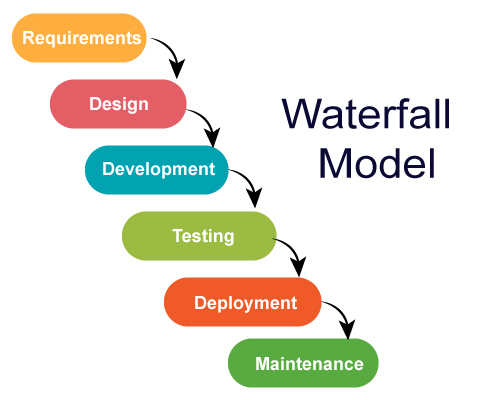
\includegraphics[width=0.35\textwidth]{waterfall-model.png}
  \caption{Modello a cascata}
  \label{fig:waterfallModel}
\end{figure}

\paragraph{Metodologia Agile} Questo modello, al contrario della metodologia Waterfall, rientra nella categoria dei modelli iterativi: ogni iterazione viene chiamata \textit{sprint} ed è di breve durata, all'incirca un paio di settimane. Ogni \textit{sprint} deve comprendere tutte le fasi necessarie per rilasciare un piccolo incremento nelle funzionalità software, come mostrato in Figura~\vref{fig:sprintAgile}. L'obiettivo di ogni iterazione è quello di consegnare al cliente software "consegnabile", ovvero funzionante e di buona qualità anche se per le funzionalità fornite non è considerabile completo. Questo al fine di coinvolgere maggiormente il cliente nel processo di sviluppo e avere la possibilità di rivalutare i requisiti e le priorità a progetto in corso, riducendo il rischio di fallimento. 

Cluster Reply utilizza questa metodologia nei casi in cui il cliente non abbia le idee perfettamente chiare riguardo i requisiti e sia necessario un metodo di lavoro più agile e aperto ai cambiamenti.

\begin{figure}[ht]
  \centering
  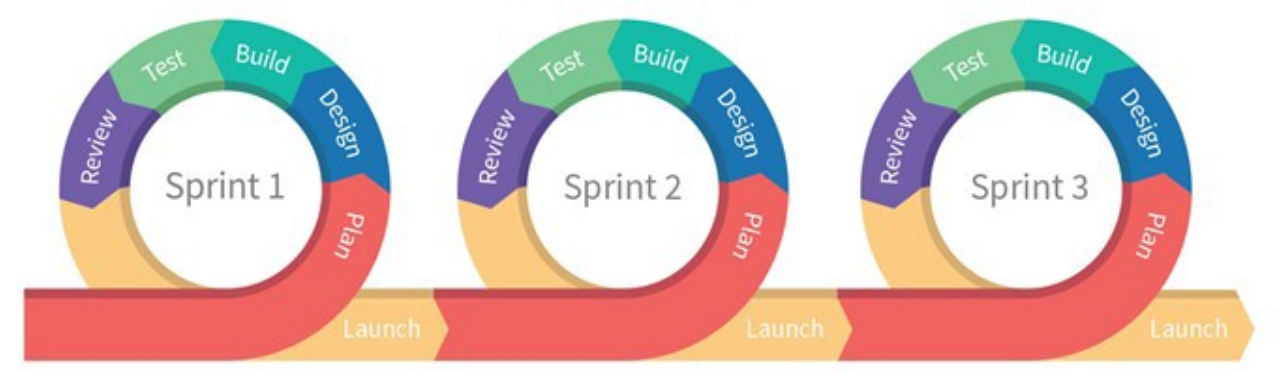
\includegraphics[width=0.50\textwidth]{agile.png}
  \caption{\textit{Sprint} nella metodologia Agile}
  \label{fig:sprintAgile}
\end{figure}

\paragraph{Metodologia Reply} Questa metodologia può essere considerata come una versione intermedia tra Agile e Waterfall in quanto fa suoi diversi aspetti sia dell'una che dell'altra. Viene mantenuta quindi una programmazione lineare e sequenziale del progetto secondo le varie fasi successive. La differenza rispetto a Waterfall, tuttavia, è che il cliente viene periodicamente coinvolto nel progetto e aggiornato sull'andamento, mostrandogli ciò che è stato fatto fino a quel momento. Il fine è quello di ridurre il rischio di fallimento del progetto evitando che il cliente si veda consegnare un prodotto diverso dalle aspettative. Durante la fase di \textit{solution review}, la revisione periodica con il cliente, è comunque possibile rivedere i piani e fare modifiche a progetto in corso, a discapito dell'efficienza e dei tempi di sviluppo e consegna del prodotto.

Si opta per questa metodologia qualora il cliente manifesti la necessità di monitorare frequentemente lo stato di avanzamento del prodotto e il tipo di progetto mal si prestasse all'utilizzo della metodologia Agile.

\setlength{\parskip}{2em}
Indistintamente dalla metodologia utilizzata, resta necessario sottolineare l'importanza delle fasi di analisi di fattibilità e dei requisiti che si concretizzano nell'elaborazione del documento di analisi funzionale. Quest'ultimo, oltre a definire cosa deve essere fatto, è un'importante tutela dell'azienda dal punto di vista commerciale ed economico in quanto stabilisce cosa il cliente ha richiesto e quindi per cosa sta pagando. Aggiunte o modifiche rispetto a quanto approvato dal cliente nel documento di analisi funzionale, sono da considerarsi non incluse nell'accordo commerciale e quindi da saldare separatamente.
\setlength{\parskip}{0em}

\section{Strumenti a supporto dei processi}
Durante le fasi di sviluppo vengono utilizzati diversi strumenti a supporto delle varie operazioni.

\subsubsection{Strumenti di gestione del progetto}
Per la pianificazione e organizzazione del progetto Cluster Reply fa largo uso di Microsoft Project. Questo software permette la creazione dei diagrammi GANTT del progetto, la definizione dei task e delle \textit{milestone} e il monitoraggio del loro stato, oltre che alla realizzazione di reportistica come i diagrammi dell'\textit{effort}. 
Per la gestione dei budget e delle giornate e orari dedicati alla consuntivazione commesse viene utilizzato invece Geco, un software interno a Reply.

\subsubsection{Strumenti di sviluppo} I linguaggi principalmente utilizzati sono C\# e .NET per lo sviluppo di plugin e azioni, a questo si aggiunge l'utilizzo delle librerie Microsoft XRM SDK e Microsoft CRM SDK.
Viene inoltre utilizzato Javascript per la parte frontend mentre per la manipolazione di database principalmente T-SQL. 
L'ambiente di sviluppo usato principalmente è Microsoft Visual Studio.
Per quanto riguarda il \textit{version control} del codice e i \textit{backlog} tecnici viene utilizzato Azure DevOps.



